% Chapter 22 -- Claim: Foundation Models Beat Classical Forecasts
% Requires: amsmath, amssymb, booktabs, array, tabularx, graphicx, tcolorbox (breakable, skins), hyperref or url.
% Defines the callout box only if the preamble has not.
\providecolor{fenavy}{HTML}{1B2A6B}
\providecolor{feshade}{HTML}{F3F5FA}
\makeatletter
\@ifundefined{callout}{%
  \newtcolorbox{callout}{breakable, enhanced,
    colback=white, colframe=gray!70, boxrule=0.5pt, arc=1mm,
    borderline west={2.5pt}{0pt}{gray!70},
    left=8pt, right=8pt, top=4pt, bottom=4pt}%
}{}
\makeatother

\chapter{Claim: Foundation Models Beat Classical Forecasts}
\label{ch:22}

Large language models learned to write by reading most of the internet. Since 2024, the same recipe has been applied to numbers. Time-series foundation models, such as Amazon's Chronos and Google's TimesFM, are pretrained on billions of observations from thousands of series: electricity demand, web traffic, weather, retail sales. They then forecast series they have never seen, with no training at all. Their developers report that, used this way, they match or beat models fitted specifically to each dataset.

For finance and economics the promise is striking: one pretrained model, applied to returns, volatility or inflation, could replace the careful work of specifying and estimating a model for each series.

Financial series are unlike most of the data these models learn from. Returns are close to unpredictable, volatility has long memory and fat tails, and macroeconomic series are short and revised. Public financial data may also have been part of the training set, which can flatter a model on history. This chapter asks whether foundation models beat simple classical benchmarks once those problems are taken seriously.

By the end of the chapter you will be able to:

\begin{itemize}
  \item name the classical benchmark for each kind of series: the historical mean, the naive forecast, autoregressions, GARCH and HAR;
  \item explain how a time-series foundation model is pretrained and used zero-shot, and how Chronos and TimesFM differ;
  \item explain contamination, and why only data published after a model's training cutoff give a clean test;
  \item evaluate forecasts on rolling origins with MSE ratios, the Diebold--Mariano test, interval coverage and the pinball and QLIKE losses;
  \item calculate how long an evaluation sample must be to detect a small gain;
  \item state the claim and judge the evidence on returns, volatility, other financial series and macroeconomic series.
\end{itemize}

\section{Foundations: benchmarks, foundation models and fair tests}
\label{sec:22-foundations}

\textbf{Classical benchmarks.} A forecasting method earns attention only if it beats simple alternatives:

\begin{itemize}
  \item The \textbf{historical mean} forecasts the average of all past values. It is hard to beat for stock returns (Chapter 7).
  \item The \textbf{naive} or random-walk forecast is the last observed value. It is hard to beat for exchange rates and interest-rate levels.
  \item An \textbf{autoregression}, AR($p$), regresses the series on its own past $p$ values:
  \begin{equation}
    y_{t+1} = c + \phi_1 y_t + \cdots + \phi_p y_{t-p+1} + \varepsilon_{t+1}
    \label{eq:22-ar}
  \end{equation}
  The number of lags can be chosen by an information criterion such as BIC. \textbf{ARIMA} models add differencing and moving-average terms.
  \item For volatility, \textbf{GARCH} models update the variance with each squared return (Chapter 11), and the \textbf{HAR} model regresses realized variance on its recent daily, weekly and monthly averages (Corsi 2009). Both capture volatility's long memory with few parameters.
\end{itemize}

\textbf{Foundation models.} A time-series foundation model is a large neural network, usually a \textbf{transformer}, pretrained on a broad collection of series and then used \textbf{zero-shot}, without any training on the target series. Two design families matter here:

\begin{itemize}
  \item \textbf{Chronos} (Ansari et al.\ 2024) scales each series and quantizes its values into a fixed vocabulary of tokens. It then trains a T5 language-model architecture to predict the next token, which yields a full probability distribution for the forecast. Models range from 20 million to 710 million parameters. Chronos-Bolt is a faster successor.
  \item \textbf{TimesFM} (Das et al.\ 2024) is a decoder-only transformer of about 200 million parameters. It reads the series in patches of consecutive points and outputs longer patches. It was pretrained on about 100 billion time points, mostly Google Trends search interest and Wikipedia page views, plus synthetic series.
\end{itemize}

The pitch is breadth: a model that has seen trends, seasonality, mean reversion and regime shifts across many domains should recognize them in a new series.

\textbf{Contamination.} A forecast evaluation is valid only if the model has not seen the test data. Classical models are fitted on past data at each forecast date, so this is easy to guarantee. A foundation model's pretraining corpus is fixed and often only partly documented. If it contains the test series, or close copies such as a stock index that tracks the target, the model may partly be remembering rather than forecasting. The clean test uses data published after the model's \textbf{training cutoff}.

\textbf{Evaluation.} Forecasts are compared on the same \textbf{rolling origins}: at each month $t$, every model forecasts month $t+1$ using only data up to $t$ (Figure~\ref{fig:22-rolling}).

\begin{itemize}
  \item The \textbf{mean squared error (MSE) ratio} divides a model's MSE by that of a benchmark; below 1 means better.
  \item The \textbf{Diebold--Mariano test} (Diebold and Mariano 1995) checks whether the average difference in squared errors is significantly different from zero.
  \item For distributional forecasts, \textbf{coverage} asks whether an 80\% interval contains the outcome 80\% of the time, and the \textbf{pinball loss} scores each quantile.
  \item For volatility, the \textbf{QLIKE} loss is robust to noise in the realized-variance proxy (Patton 2011; Section~\ref{sec:11-eval}).
\end{itemize}

\begin{figure}[htbp]
\centering
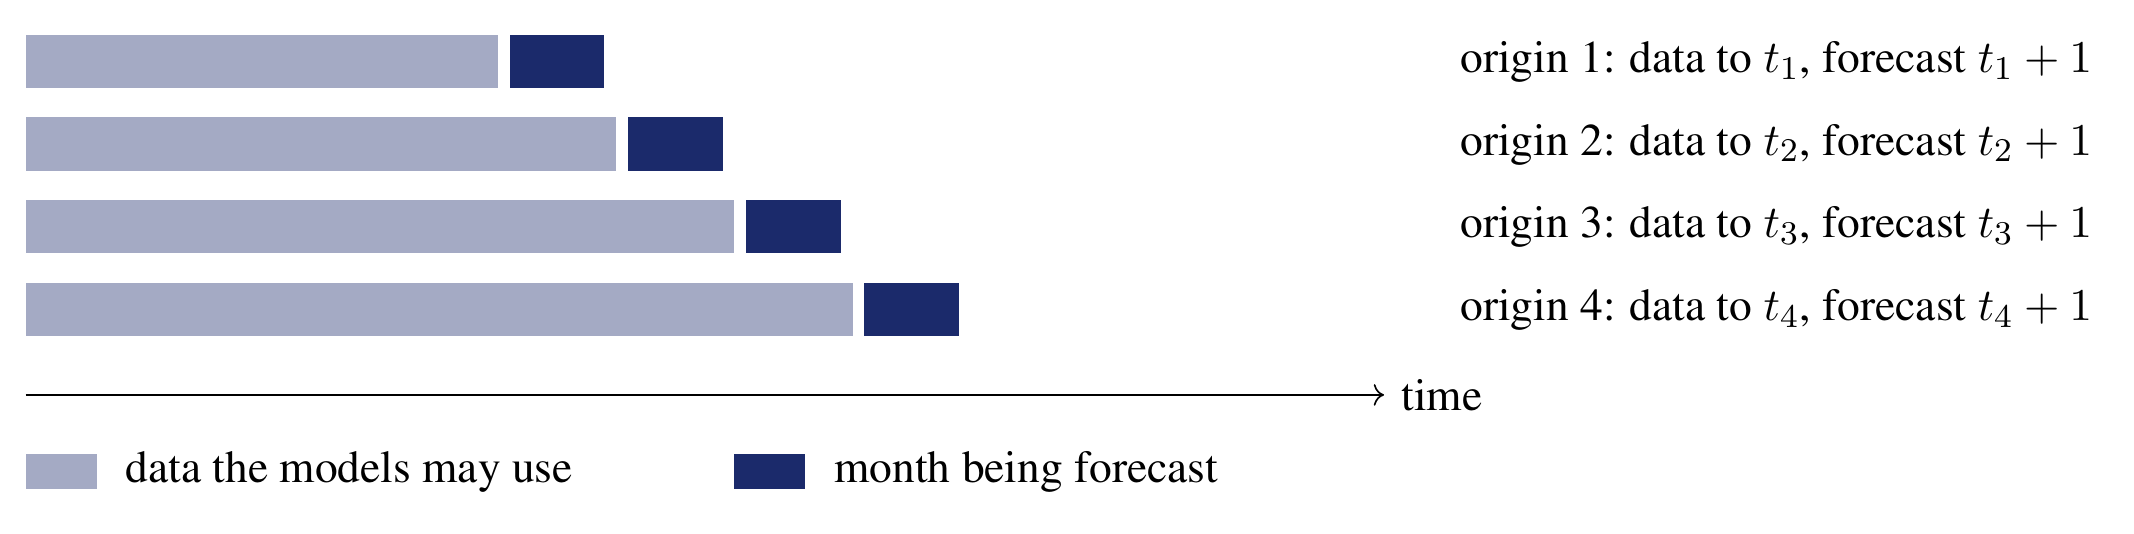
\includegraphics[width=0.85\linewidth]{images/fig22-1-rolling.png}
\caption{Rolling-origin evaluation. At each origin every model sees the same data up to that month and forecasts the next one; the origin then moves forward a month. No model ever sees the month it is forecasting.}
\label{fig:22-rolling}
\end{figure}

\textbf{Worked example.} Suppose an AR model's one-month inflation forecasts have an MSE of 0.040 (percentage points squared) over 300 months and a foundation model's 0.038.

\begin{itemize}
  \item The MSE ratio is 0.95, a 5\% gain.
  \item If the monthly loss differences have a standard deviation of 0.020 and little autocorrelation, the Diebold--Mariano statistic is $0.002 / (0.020/\sqrt{300}) \approx 1.7$, not significant at 5\%.
  \item A gain of that size needs a long evaluation sample to be distinguished from luck, and a post-cutoff window of two years has only 24 observations (Figure~\ref{fig:22-dm}).
\end{itemize}

\begin{figure}[htbp]
\centering
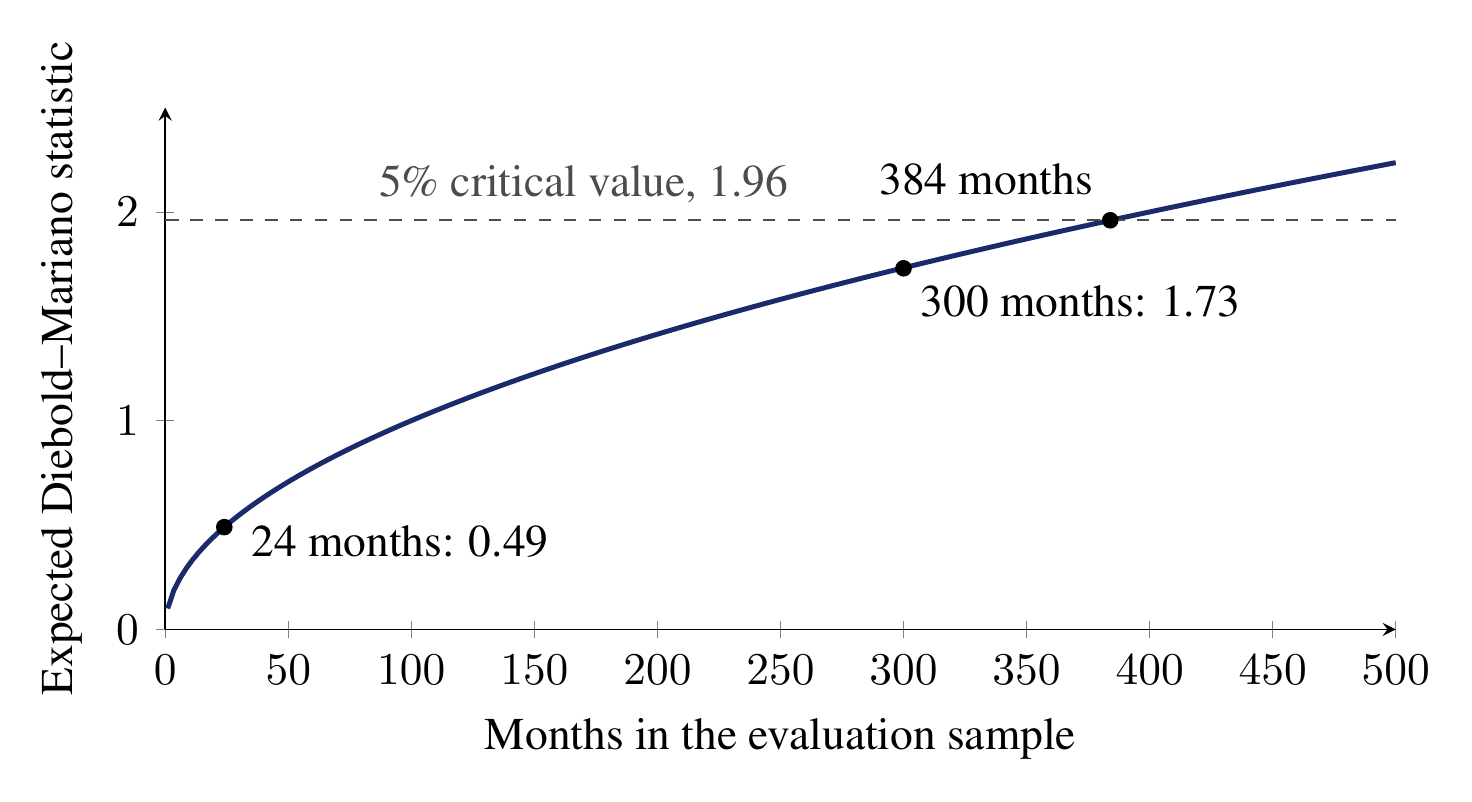
\includegraphics[width=0.85\linewidth]{images/fig22-2-dm-power.png}
\caption{The expected Diebold--Mariano statistic for the worked example's 5\% gain, as the evaluation sample grows. It reaches 1.96 only after about 384 months; a two-year post-cutoff window gives about 0.5.}
\label{fig:22-dm}
\end{figure}

\textbf{Further reading.} Hyndman and Athanasopoulos, \emph{Forecasting: Principles and Practice}, and Diebold, \emph{Elements of Forecasting} (forecasting principles and classical methods); Hamilton, \emph{Time Series Analysis}, and Tsay, \emph{Analysis of Financial Time Series}; Elliott and Timmermann, \emph{Economic Forecasting} (forecast evaluation); Goodfellow, Bengio and Courville, \emph{Deep Learning} (transformers and pretraining).

\section{How it works}
\label{sec:22-how}

A zero-shot forecast takes three steps. The recent history of a series, up to a few hundred observations, is normalized and passed to the pretrained network. The network outputs a forecast for the next step or steps, often as a set of quantiles. Nothing is estimated on the target series; all the knowledge comes from pretraining.

That design has clear strengths:

\begin{itemize}
  \item \textbf{No specification work.} There are no lags to choose and no model to estimate.
  \item \textbf{Short histories.} Patterns learned elsewhere can fill in for a lack of data on the target series.
  \item \textbf{Probabilistic output.} Forecast intervals come built in.
\end{itemize}

It also has limits that bite hardest in finance:

\begin{itemize}
  \item \textbf{Weak signal.} Most of the variation in a monthly return is noise. A model trained to extend patterns may find them where none exist.
  \item \textbf{Domain mismatch.} Pretraining corpora are dominated by series with strong seasonality and trends: energy demand, traffic, sales. Financial returns have neither, and volatility has dynamics that few other series share.
  \item \textbf{Scale and context.} Normalizing each window discards the level of a series. For volatility or inflation, the level itself carries information about what comes next.
  \item \textbf{Contamination.} Popular financial and macroeconomic series are widely published, so a model may have seen them, or close relatives, in pretraining.
\end{itemize}

Classical models are the opposite: narrow, but fitted to the target series and transparent about what they assume. The question is whether breadth beats fit.

\section{The claim}
\label{sec:22-claim}

\begin{callout}
\textbf{Claim.} Pretrained time-series foundation models, used zero-shot, forecast financial and economic series better than classical models.
\end{callout}

To count as evidence, a test must:

\begin{itemize}
  \item compare against strong classical benchmarks for each series (the historical mean for returns, AR models for macroeconomic series, HAR for realized volatility), not only against naive forecasts;
  \item use rolling origins, with each forecast made only from data available at the time;
  \item report significance, not just average losses;
  \item show that the result holds on data the model cannot have seen during pretraining.
\end{itemize}

\section{The original evidence}
\label{sec:22-evidence}

\textbf{The developers' benchmarks.}

\begin{itemize}
  \item \textbf{Chronos (Ansari et al.\ 2024).} Chronos was pretrained on a large collection of public datasets plus synthetic series generated from Gaussian processes, and evaluated on 42 datasets. On datasets that were part of its training corpus, it significantly outperformed other methods. On new datasets, its zero-shot performance was comparable to, and occasionally better than, models trained on those datasets.
  \item \textbf{TimesFM (Das et al.\ 2024).} Google reported that TimesFM beat statistical methods such as ARIMA and ETS on unseen data, and matched or beat deep-learning models trained on the target series, on standard benchmark archives.
\end{itemize}

These benchmarks contain few financial series. The Chronos result also illustrates the contamination problem: performance was strongest on data the model had seen.

\textbf{Daily stock returns (Rahimikia, Ni and Wang 2025).} Rahimikia, Ni and Wang tested Chronos, TimesFM and other foundation models on daily excess returns of securities in 94 countries from 1990 to 2023, out of sample from 2001. Off-the-shelf models performed poorly. Zero-shot Chronos (large) had an out-of-sample $R^2$ of $-1.37\%$, with about 51\% directional accuracy, and TimesFM had $-2.80\%$. Fine-tuning helped little. Pretraining the same architectures from scratch on financial data improved them substantially, but they still trailed tree ensembles such as CatBoost on $R^2$. The authors concluded that generic pretraining does not transfer directly to finance.

\textbf{Multivariate financial series (Marconi 2025).} Marconi evaluated Tiny Time Mixers and Chronos on changes in the U.S. 10-year Treasury yield, EUR/USD volatility and an equity spread. Zero-shot, the models beat naive baselines on volatility and the spread. Fine-tuning a pretrained model beat training the same architecture from scratch, and needed several fewer years of data. But specialised traditional models matched or beat the foundation model on two of the three tasks.

\textbf{Realized volatility (Brini 2026).} Brini compared nine zero-shot foundation models with eight econometric models, including HAR variants and ARFIMA. The data were daily realized volatility for 40 U.S. stocks, five currency pairs and five futures contracts, at horizons of 1, 5 and 22 days. Pooled losses favoured the foundation models, but the advantage came from a few outlier assets. On average per-asset QLIKE loss, only one model (Tiny Time Mixers) beat a log-HAR benchmark at every horizon, by about 1.3\% to 1.8\%; the other eight did not. An equal-weight average of that model and log-HAR was among the best forecasts for almost every asset.

The pattern across studies is consistent. Zero-shot foundation models beat naive forecasts easily, sometimes match well-specified classical models, and rarely beat them by a meaningful margin. Where they do, combining them with a classical model helps more than replacing it.

\section{Replication lab: six series, one month ahead}
\label{sec:22-lab}

\begin{callout}
\textbf{Lab 22 at a glance.} \emph{Claim on trial:} foundation models, used zero-shot, beat classical forecasts. \emph{Data:} the U.S. market's excess return and its log realized variance built from daily returns (Kenneth R. French Data Library); inflation, industrial production growth, and the changes in the unemployment rate and in the 10-year Treasury yield (FRED). All are free. \emph{Code:} runs as a script (\texttt{python lab22.py -{}-models chronos-bolt-small timesfm}) or as a notebook (\texttt{lab22\_walkthrough.ipynb}) with a prediction prompt before each step.
\end{callout}

Lab 22 forecasts the six series one month ahead, from every month since January 2000. At each month, every model sees only data up to that month.

\begin{center}
\small
\begin{tabularx}{0.9\linewidth}{@{}>{\raggedright\arraybackslash}X>{\raggedright\arraybackslash}p{0.38\linewidth}@{}}
\toprule
Model & Type \\
\midrule
Historical mean & Classical \\
Naive (last value) & Classical \\
AR, lags chosen by BIC on the last 30 years & Classical: \textbf{the benchmark} \\
HAR-type: last value, 3-month and 12-month averages & Classical \\
GARCH(1,1), realized variance only & Classical \\
Chronos-Bolt (small and base) & Foundation model, zero-shot \\
TimesFM & Foundation model, zero-shot \\
\bottomrule
\end{tabularx}
\end{center}

The foundation models are optional, because they need PyTorch and large model downloads (\texttt{pip install chronos-forecasting timesfm}). Without them, the lab runs everything else and reports which models could not be loaded.

The lab has four parts:

\begin{itemize}
  \item \textbf{Part A} reports each model's MSE relative to AR, and its $R^2$ against the historical mean (Figures 22.3 and 22.7).
  \item \textbf{Part B} adds Diebold--Mariano tests, the share of months each model beats AR and the cumulative squared-error difference over time (Figure 22.4).
  \item \textbf{Part C} splits the evaluation at a cutoff date, by default January 2024, to be set to each model's training cutoff. A deliberately contaminated ``memorizing'' model, which is shown the answer before the cutoff, displays the signature of contamination (Figure 22.5).
  \item \textbf{Part D} checks whether each model's 80\% forecast intervals contain the outcome 80\% of the time (Figure 22.6).
\end{itemize}

The command \texttt{python lab22.py -{}-source sim -{}-models standin} tests the code.

\textbf{What the simulated run shows.} The lab was run end to end only on simulated data, and without any foundation model. A clearly labelled stand-in, the average of three classical forecasts, took the foundation models' place. The results test the code and illustrate the evaluation, not the models.

\begin{itemize}
  \item For simulated returns, which are unpredictable by construction, the historical mean beat AR (MSE ratio 0.98) and the naive forecast doubled the error (1.99).
  \item For simulated log realized variance, which has long memory, HAR and AR were nearly tied (0.996), the historical mean was nine times worse, and GARCH on monthly returns was almost three times worse. GARCH sees only one return a month, while the realized-variance models see daily data.
  \item The stand-in never beat AR significantly; it was worse on five of six series, by up to 12\%.
  \item The memorizing model had an MSE ratio of 0.16 before the cutoff and exactly 1.00 after it. That collapse is what contamination looks like.
  \item The AR and HAR-type models' 80\% intervals contained the outcome 79\% to 81\% of the time; the historical mean's interval for realized variance managed only 53\%.
\end{itemize}

Run with the foundation models on real data, the lab answers the chapter's question directly: whether they beat AR and HAR, whether their edge survives the cutoff and whether their intervals are honest.

\section{Stress tests}
\label{sec:22-stress}

\textbf{Benchmark strength.} Most claims of superiority are made against naive forecasts or against classical models that were not tuned for the target series. Against the historical mean for returns, AR for macroeconomic series and HAR for volatility, the gap narrows or disappears.

\textbf{Contamination.} The only clean evaluation is on data published after the model's training cutoff. Developers rarely list every series in their corpora, so cutoff dates are often approximate. A post-cutoff window of a year or two is short for monthly data, and significance tests will have little power.

\textbf{Frequency and horizon.} Studies of daily realized volatility at horizons of 1 to 22 days find small, uneven gains. Monthly series give far fewer observations. Gains may appear at some horizons and not others, so results should be reported by horizon.

\textbf{Pooled versus per-series results.} A model can win on pooled losses because of a few series with large errors while losing on most series. Brini's realized-volatility study found exactly that. Per-series results, or losses scaled to each series, avoid the problem.

\textbf{Model versions.} Foundation models are updated often, and results for one version may not hold for the next. Evaluations should name the exact model and version.

\textbf{Context length.} Foundation models normalize each input window. Giving them 64 rather than 512 months of history can change both the forecast and its interval.

\section{Verdict}
\label{sec:22-verdict}

\begin{callout}
\textbf{Verdict: provisional} (as of October 2026). The evidence so far does not support the claim, but it is too new and too thin to reject it.
\end{callout}

\begin{itemize}
  \item \textbf{Returns.} Zero-shot foundation models forecast stock returns worse than simple benchmarks (Rahimikia, Ni and Wang 2025). Pretraining on financial data helps, which suggests the problem is the domain, not the architecture.
  \item \textbf{Volatility.} Most foundation models do not beat a well-specified HAR model on average. The best one beats it by one or two percent, and the most reliable forecast combines the two (Brini 2026).
  \item \textbf{Other financial series.} Foundation models beat naive baselines but are matched or beaten by specialised models in most tasks studied (Marconi 2025).
  \item \textbf{Macroeconomic series.} Clean, post-cutoff evaluations are still scarce.
\end{itemize}

The field changes quickly, and models pretrained on financial data are appearing. The verdict should be revisited when there are post-cutoff evaluations of several years for the main financial and macroeconomic series. It would move to \emph{survives} if a foundation model beat AR and HAR significantly on data it cannot have seen, and to \emph{fails} if successive generations continued to fall short of them.

\section{What investors can use}
\label{sec:22-investors}

\begin{itemize}
  \item \textbf{Benchmark before you buy.} Any forecasting tool, foundation model or not, should be compared with the historical mean for returns, an autoregression for macroeconomic series and HAR for volatility, on the same rolling origins.
  \item \textbf{Use foundation models as a second opinion.} The most consistent finding is that averaging a foundation model with a classical model beats either alone. Combination is cheap and reduces the risk of relying on one model's quirks.
  \item \textbf{Be strict about dates.} Ask when the model's training data end. Treat any evaluation on earlier data as possibly contaminated.
  \item \textbf{Value speed honestly.} Zero-shot models are quick to deploy across many series. That convenience is real, but it is not the same as accuracy, and a classical AR model is also quick.
  \item \textbf{Check the intervals.} A model whose 80\% intervals cover the outcome far less than 80\% of the time understates risk.
\end{itemize}

\textbf{Questions to ask a vendor or team proposing a foundation-model forecast:}

\begin{itemize}
  \item Which classical benchmarks did you compare against, and were they tuned for each series?
  \item What is the model's training cutoff, and how does performance compare before and after it?
  \item Are results reported per series and per horizon, or only pooled?
  \item Which exact model version produced the results, and will it change?
  \item How well calibrated are the forecast intervals?
\end{itemize}

\begin{callout}
\textbf{What Failed: forecasting home prices at scale.} In 2018 Zillow began buying homes directly through Zillow Offers, relying on its price-estimation models to decide what to pay and expecting to resell at a profit. In November 2021 the company announced it would wind the business down (Zillow Group 2021). It wrote down its home inventory by \$304.4 million in the third quarter, having bought homes at prices above what it now expected to sell them for, and cut about a quarter of its workforce. Zillow cited home pricing unpredictability, capacity constraints and other operational challenges. The models were sophisticated and trained on vast data, but a forecast that is accurate on average can still fail when it is acted on at scale, in a market that turns, against counterparties who know more about the specific asset. The lesson for any new forecasting technology is to test it where the decision is made, not where the benchmark is easiest.
\end{callout}

\section{Open questions}
\label{sec:22-open}

\begin{itemize}
  \item \textbf{Finance-specific pretraining.} Will models pretrained on large financial datasets beat classical and tree-based benchmarks out of sample, and by enough to matter after costs?
  \item \textbf{Clean evaluation.} Can the field agree on post-cutoff benchmarks for financial and macroeconomic series, so that each new model is tested on data it cannot have seen?
  \item \textbf{Multivariate and conditional forecasts.} Most zero-shot tests are univariate. Can foundation models use related series, such as option-implied volatility for realized volatility, as classical models can?
  \item \textbf{Language and numbers.} Large language models can read news and filings. Does combining text with time-series models improve forecasts of returns, volatility or the economy? Chapter 23 takes up the text half.
\end{itemize}

\section*{Exercises}
\addcontentsline{toc}{section}{Exercises}

\subsection*{Conceptual (all readers)}

\begin{enumerate}
  \item A foundation model's MSE ratio against AR is 0.97 over 120 months. The monthly loss differences have a standard deviation 4 times their mean. Compute the Diebold--Mariano statistic, ignoring autocorrelation. How many months would be needed for the same gain to reach $t = 2$?
  \item Explain why the historical mean is a strong benchmark for monthly stock returns but a weak one for log realized variance.
  \item A foundation model was pretrained on a corpus that includes the S\&P 500 index up to 2023. Which of the lab's six series could be affected, and why?
\end{enumerate}

\subsection*{Lab extensions (technical readers)}

\begin{enumerate}
  \setcounter{enumi}{3}
  \item Install Chronos-Bolt and run the lab on real data. On which series does it beat AR, and is any difference significant?
  \item Compare Chronos-Bolt with HAR on log realized variance. Then average the two forecasts. Does the average beat both?
  \item Part C: set the cutoff to Chronos-Bolt's release date. How do its MSE ratios before and after compare with the memorizing model's pattern?
  \item Part D: check the 80\% interval coverage of the foundation models. Are their intervals too narrow, too wide or about right?
  \item Chronos performed best on datasets that were in its training corpus. Why does that make developers' benchmark results hard to interpret for financial users?
  \item A colleague argues that because foundation models are improving quickly, it is not worth building classical benchmarks. Write a short reply.
\end{enumerate}

\section*{References}
\addcontentsline{toc}{section}{References}

\begin{itemize}
  \item Ansari, A. F., et al.\ (2024). Chronos: Learning the Language of Time Series. \emph{Transactions on Machine Learning Research}.
  \item Brini, A. (2026). Forecasting Realized Volatility with Time Series Foundation Models: A Comparison with Econometric Benchmarks. arXiv:2607.05291.
  \item Corsi, F. (2009). A Simple Approximate Long-Memory Model of Realized Volatility. \emph{Journal of Financial Econometrics} 7(2): 174--196.
  \item Das, A., Kong, W., Sen, R. and Zhou, Y. (2024). A Decoder-Only Foundation Model for Time-Series Forecasting. \emph{Proceedings of the 41st International Conference on Machine Learning}.
  \item Diebold, F. X. and Mariano, R. S. (1995). Comparing Predictive Accuracy. \emph{Journal of Business \& Economic Statistics} 13(3): 253--263.
  \item Marconi, B. A. (2025). Time Series Foundation Models for Multivariate Financial Time Series Forecasting. arXiv:2507.07296.
  \item Patton, A. J. (2011). Volatility Forecast Comparison Using Imperfect Volatility Proxies. \emph{Journal of Econometrics} 160(1): 246--256.
  \item Rahimikia, E., Ni, H. and Wang, W. (2025). Re(visiting) Time Series Foundation Models in Finance. arXiv:2511.18578.
  \item Zillow Group (2021). Form 8-K, November 2, 2021.
\end{itemize}

\textbf{Data:} Kenneth R. French Data Library: Fama/French 3 Factors, monthly and daily. FRED, Federal Reserve Bank of St.\ Louis: Consumer Price Index [CPIAUCSL], Industrial Production [INDPRO], Unemployment Rate [UNRATE], 10-Year Treasury Constant Maturity Rate [GS10].
